\setchapterpreamble[u]{\margintoc}
\chapter{Creativity and Decision Making with Deep Learning Models}
\labch{decisions}

\textit{"AI Policy}

\textit{I expect you to use AI (ChatGPT and image generation tools, at a minimum), in this class. In fact, some assignments will require it. Learning to use AI is an emerging skill, and I provide tutorials in Canvas about how to use them. I am happy to meet and help with these tools during office hours or after class}

\textit{Beware of the limits of ChatGPT:}

\begin{itemize}
	\item\textit{If you provide minimum effort prompts, you will get low quality results. You will need to refine you prompts to get good outcomes. This will take work.}
	\item\textit{Don't trust anything it says. If it gives you a number or a fact, assume it is wrong unless you either know the answer or can check in with another source. You will be responsible for any errors or omissions provided by the tool. It works best for topics you understand.}
	\item\textit{AI is a tool, but one that you need to acknowledge using. Please include a paragraph at the end of any assignment that uses AI explaining what you used the AI for and what prompts you used to get the results. Failure to do so is in violation of academic honesty policies}
	\item\textit{Be thoughtful about when this tool is useful. Don't use it if it isn't appropriate for the case or circumstance."}
\end{itemize}

\textit{Dr. Ethan Mollick, 2023 - Syllabus for class at The Wharton School at the University of Pennsylvania}


\section{Theories of Creativity}

Machine learning models use data (from the past) to discover rules and make classifications. Because of the way they are constructed these classifications, suggestions, artworks are by definition derivative or "having parts that originate from another source". I won't get into a philosophical discussion on what the nature of creativity is, but it's worth considering how using deep learning models biases us towards the past, but also could give us insights from other domains. 

\begin{marginfigure}[-5.5cm]
        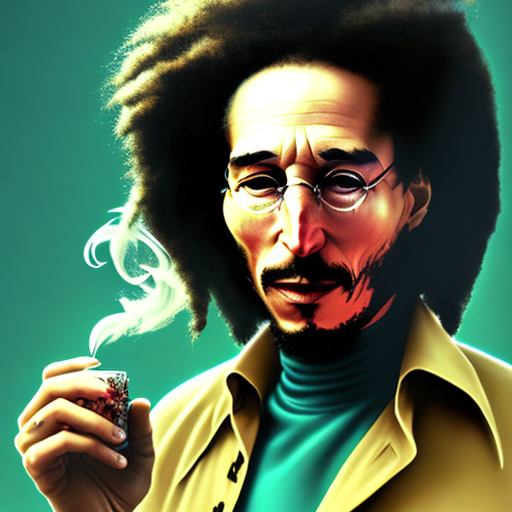
\includegraphics{jobsweed}
        \caption{"mdjrny-v4 Steve Jobs Smoking weed with Bob Marley 8k" made with Mann-E. It's 100\% derivative, but it's art too (I guess).}
        \labfig{jobsweed}
\end{marginfigure}

It can be argued that creativity is simply the combination of existing works. This is because many new ideas and innovations are often inspired by and built upon existing concepts. For example, a new form of music may be created by combining elements from different genres. Similarly, a new technology may be created by combining and improving upon existing technologies.

It can also be argued that creativity involves much more than just combining existing works. Creativity is not just about recombining existing ideas, but also about coming up with completely new and original concepts. This requires a unique perspective and a deep understanding of the subject matter, as well as the ability to think outside the box.  

Deeep learning models of speech, when heavily used, may slow down the evolution of language. AI art models may slow down "progress" in art, whatever that means. Deep learning models of disease trained on data from 1980 may be irrelevant to today's diseases. That said these same models may give us interesting insights in new domains, models trained on beautiful paintings may be put to use in a new domain (like designing beautiful interiors) and that model could give new insight to interior designers, models of the interaction of ants could be put to use in designing cities and so on and so forth. AI cuts many ways, it makes us faster but makes us more reliant on the past, models can be used across domains but should be used intentionally and transparently when possible. Each use opens up a new world of possibilities for users, and sometimes a new headache for intellectual property lawyers. We'll discuss all of these topics in this chapter.

\begin{marginfigure}[-5.5cm]
        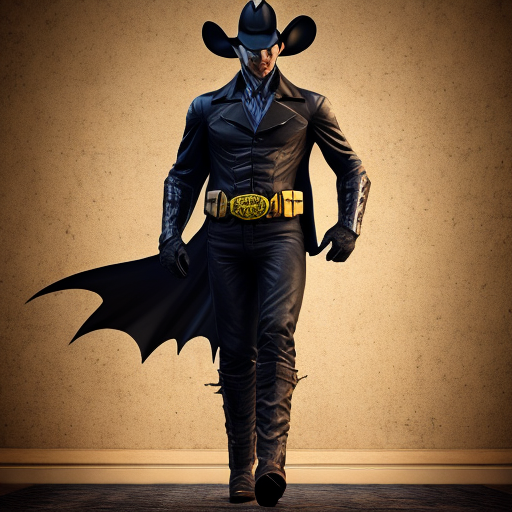
\includegraphics{batman}
        \caption{"Batman dressed as a cowboy" made with Mann-E. It's 100\% derivative as well, but better than any Google image searches I did. It looks amazing! I also might get sued if I use it even though the creators of Mann-E tell me I have the rights to it.}
        \labfig{batman}
\end{marginfigure}

\section{Creative Uses of Power Tools}

Power tools, even simple ones like a drill are complex machines that take human input and transform it using static rules. The pressure the user of a drill puts on the bit and the speed at which they pull the trigger all deterministically affect the output. Just because a tool is a deterministic machine doesn't mean it is unable to produce creative works.

What is happening as we use generative tools like ChatGPT or image-to-text models is that the "creative act" has been relocated. The creative act is now the prompt you give the tool, the users input. And someone can still be good at using AI, just like someone can be good at using any piece of software.

Modern AI is a complex system of algorithms, data, and analytics that can be used to solve complex problems. AI systems can learn from data, identify patterns, and make predictions about the future. AI systems are typically used to automate and assist human decision making. AI systems are programmed with specific objectives and goals, and the user input decides the output. For example, an AI system could be programmed to solve a mathematical problem and the user input would determine the parameters of the problem and the output would be the solution.

A power drill is also a complex deterministic system. The user input is limited to the type of drill bit, the speed of the drill, and the direction of the drill. The output is determined by these inputs, as the drill will only drill in the direction and speed determined by the user. The user also has to choose the correct drill bit to ensure the drill can do the job correctly and safely.

\begin{marginfigure}[-5.5cm]
        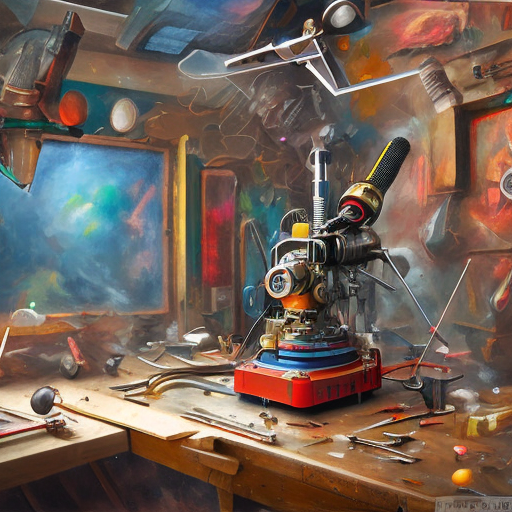
\includegraphics{drillart}
        \caption{"mdjrny-v4 a mikita drill being used in an artist's studio to make a colorful artwork 8k" made with Mann-E}
        \labfig{drillart}
\end{marginfigure}

Both modern deep learning models and a power drill are complex but ultimately deterministic systems. The user input, however limited it may be, ultimately controls the output of the system. Both systems require a user to understand how to use them and to make the correct input to get the desired output.

\section{Garbage In, Garbage Out}
\labsec{creative}

The "Power Tool" of AI is a deterministic, static and unchanging system and the rules of that system are determined by the data that the model is shown. If a model is trained on bad data, it will produce poor results. End of book...

... maybe not. It's worth thinking about this for a moment. It is often said that modern AI can "generalize and make informed inferences given new data". If deep learning models are really just a big regression, these models will always come up with an answer, but if the world changes, these models will still be projecting complicated averages of their past data into the future. 

So, let's separate AI's decision making into two extremes; \textit{Creative Decision Making} and \textit{Critical Decision Making}. The stakes are very low in a world of \textit{Creative Decision Making} and who cares if the AI is all a regression, and it just mushes together the limited data that it's seen. In a creative context you can also ask an AI interesting questions, so long as you don't solely rely on it's output without checking the facts first\sidenote{See the syllabus note from Dr. Mollick at the beginning of this chapter.}. Even if "Garbage In, Garbage Out" holds, garbage can still be helpful for a creative process. 

Note that this book is called "Full-Self Driving, Skynet..", a self-driving car and a nuclear-bomb-equipped all-seeing AI are clearly not engaging in any \textit{Creative Decision Making}. 

\section{Garbage In, New Perspective Out?}

For creative tasks, it generally doesn't matter that a deep learning model is unscientific or trained on a lopsided dataset. An informed user of AI knows this and can account for that in their decision making, especially when engaging in creative decision making. The situation becomes problematic once we allow deep learning models to engage in critical decision making by themselves. 

\begin{marginfigure}[-5.5cm]
        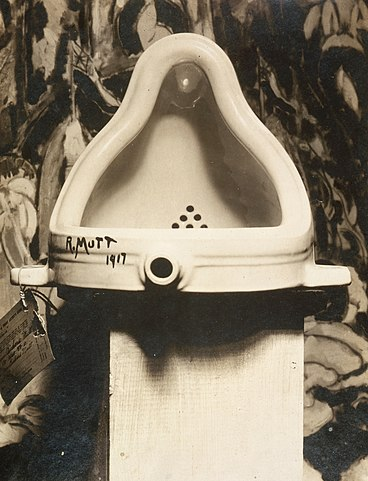
\includegraphics{duchamp}
        \caption{Marcel Duchamp's "Fountain". A urinal that blew peoples minds \url{https://www.tate.org.uk/art/artworks/duchamp-fountain-t07573}.}
        \labfig{duchamp}
\end{marginfigure}

Generative models will come up with amazing (but derivative) works of art, But, they will never "change the game". A model of sculpture trained on past sculptures in 1917 will never come up with Marcel Duchamp's "Fountain". There is a term that machine learning engineers use for this, when the rules of the game are changed, it's called "Concept Drift".

\section{Concept Drift and the End of Usefulness}
\labsec{drift}

Concept drift refers to the phenomenon where the distribution of data changes over time, causing the performance of deep learning models built on historical data to degrade. The model becomes less useful because it is trained to make predictions based on the relationship between the inputs and outputs in the data it was trained on, and if this relationship changes, the model may start making incorrect predictions. This is particularly problematic in real-world applications, where the data is constantly evolving and the relationship between inputs and outputs is subject to change. To mitigate the effects of concept drift, it is often necessary to continually retrain deep learning models on updated data.

The frequency with which a deep learning model needs to be retrained to mitigate the effects of concept drift depends on several factors, including the rate at which the data distribution changes, the size and complexity of the model, and the availability of computational resources.

For some applications with relatively stable data distributions, retraining the model once every few months or even once per year may be sufficient. However, in other applications where the data is changing rapidly, it may be necessary to retrain the model more frequently, such as once per week or even once per day.

\begin{marginfigure}[-5.5cm]
        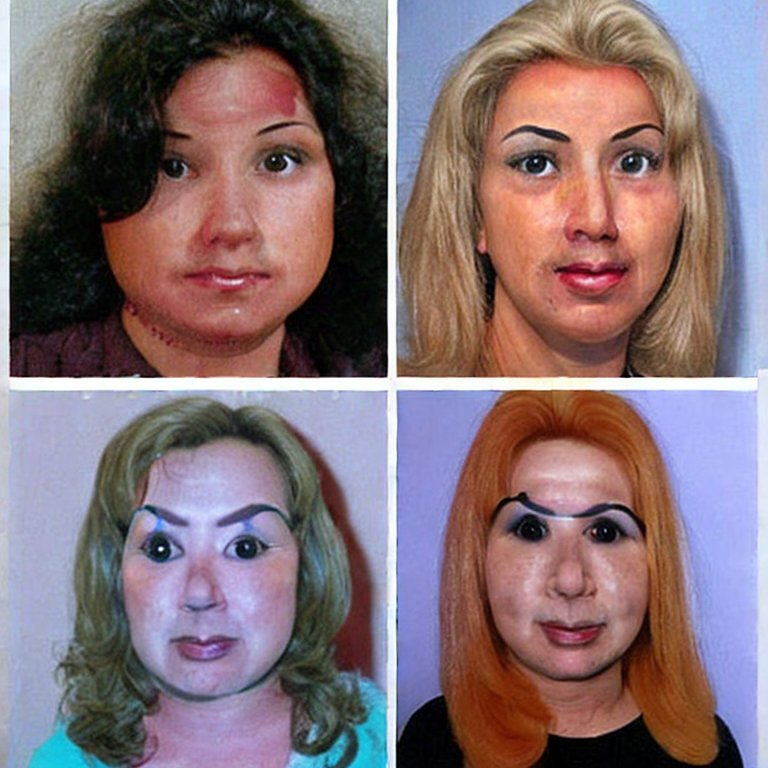
\includegraphics{plastic}
        \caption{"Plastic surgery gone wrong" made with Stable Diffusion. Imagine a model that classifies images as "human face" or "not human face", and imagine that model was trained on images of human faces before 1900, maybe you would not be surprised if you gave it a picture of a human face that had a lot of cosmetic surgery done to it, and that model might say "this is not a human face", the idea of what a human face is has changed over time this is called "concept drift".}
        \labfig{plastic}
\end{marginfigure}

Ultimately, the frequency of retraining will depend on the specific requirements of the application, and the trade-off between the cost of retraining and the potential cost of incorrect predictions. In general, it's recommended to monitor the performance of the model over time and to retrain it as needed to ensure that it remains accurate and relevant.

If a deployed deep learning model is not monitored, there are several risks that can emerge:

\begin{itemize}
\item Accuracy degradation: As the data distribution changes over time, the model may become less accurate, leading to incorrect predictions. This can result in financial losses, reduced customer satisfaction, or even harm to individuals.
\item Bias amplification: deep learning models can be biased, and if this bias is not monitored and addressed, it can be amplified over time as the model continues to make incorrect predictions. This can result in discriminatory outcomes, such as unequal treatment of individuals based on protected characteristics such as race, gender, or age.
\item Legal liability: In some cases, incorrect predictions made by deep learning models can result in legal liability, particularly if the model is being used to make decisions that have significant consequences, such as in the criminal justice system or in medical diagnosis.
\item Reputational damage: If a deep learning model is making incorrect predictions, it can damage the reputation of the organization deploying the model, potentially leading to a loss of customers or investors.
\end{itemize}


It is important to monitor deep learning models once they are deployed, and to take action to address any issues that arise, such as retraining the model or adjusting its parameters, in order to mitigate these risks and ensure that the model continues to perform well over time.

\section{The Impossibility of Fairness}

Achieving fairness in deep learning models can be challenging, and to some extent it may be impossible to completely eliminate all forms of bias. This is because deep learning models are trained on historical data, which may contain biases and disparities that are perpetuated in the model's predictions. One can attempt to "fix the training set" but in practice models will continue to bias their prediction to past data, or their creators careful curation of the past.\sidecite{Christian2020} 

However, it is possible to reduce the impact of bias in deep learning models through careful design and monitoring of the model's performance. This may include techniques such as fairness constraints, algorithmic transparency, and regular auditing of the model's predictions to identify and address any issues of bias.

It's important to note that fairness is a complex and multi-faceted concept, and different definitions of fairness may be appropriate for different applications. For example, some definitions of fairness may prioritize equal treatment of all individuals, while others may prioritize proportional representation or equal opportunities.

Ultimately, the extent to which fairness is achievable in deep learning models will depend on the specific requirements of the application and the level of effort that is put into designing and monitoring the model to ensure that it is making fair and unbiased predictions.

\section{Transfer Learning Everywhere}

Transfer learning is a machine learning technique that involves transferring knowledge from one model trained on a task to another model trained on a related task. The idea behind transfer learning is that a model that has been trained on one task can be fine-tuned for another task, reducing the amount of labeled data required to train the new model.

For example, imagine that you have a deep learning model that has been trained to recognize objects in natural images (cats, dogs, balls, cars). You can use the knowledge learned by this model as a starting point to train a new model that recognizes objects in medical images, such as X-rays or MRI scans. The new model can start with the weights of the pre-trained model and fine-tune them on the new task, using a much smaller amount of labeled data than would be required to train the model from scratch.

Transfer learning can be useful in many different applications, particularly when labeled data is scarce or expensive to obtain. By leveraging knowledge from a pre-trained model, transfer learning can help to improve the performance of new models, reduce the amount of data required for training, and accelerate the development of new machine learning applications.

I asked ChatGPT to "tell me a story of transfer learning going horribly wrong in the context of online dating, with a model trained in the Middle East being deployed by an American dating app." and here's what it said:

\textit{"Once upon a time, an American online dating company decided to use transfer learning to improve their matchmaking algorithms. They trained a state-of-the-art machine learning model on a large dataset of profiles and dating preferences from the Middle East. The model was able to suggest matches with remarkable accuracy and the company was confident that it would perform just as well in the American market.}

\textit{However, things went terribly wrong when they deployed the model on their American dating app. The model was not properly trained to consider the cultural and social differences between the Middle East and America. As a result, it suggested matches that were inappropriate and offensive, causing widespread backlash and criticism from users.}

\textit{For example, the model suggested matches between people of different religious backgrounds, which was not acceptable to many users. It also suggested matches between people with significant age gaps, which was not socially acceptable in the American market.}

\textit{The company was forced to remove the model and start from scratch, causing significant harm to their reputation and financial losses. They learned the hard way that transfer learning can only be effective if the model is properly trained on relevant and culturally appropriate data.}

\textit{This story serves as a cautionary tale about the importance of considering cultural differences and ethical implications when deploying machine learning models in different regions and markets."}

Not bad I think... picking good training data and doing good "data janitoring" is the main job of a machine learning engineer\sidenote{The better your machine learning engineer understands your business problem, the better job they'll do at creating the dataset.}.

If the past is not like the future, you are also doing transfer learning. Most models steal data from other sources so are doing transfer learning too. This is fine, but do we know that we are doing this? A model that is deployed in a domain experiencing concept drift and continues to make predictions without being retrained can be considered to be doing a harmful form of transfer learning. This is because the model has been trained on a different distribution of data (the past), and is being applied to a new domain with a different distribution (the present and future).

In traditional transfer learning, the goal is to transfer knowledge from one domain to another related domain, where the data distributions are similar enough to enable the model to make accurate predictions. However, in the case of concept drift, the data distributions are changing over time, and the model is becoming less accurate as a result. \sidenote{Think about your life and if you "transferred" your model of thinking from when you were 12 years old, to "today" when you are 35 years old, that is a bad model to be operating on! That model needs to be updated. We'll explore many examples of where this is and is not a problem in the next chapter."}

By continuing to make predictions without being retrained, the model is essentially "transferring" its knowledge from a historical data distribution to a new, changed data distribution, which may not be a valid assumption. This can result in incorrect predictions and other negative outcomes, such as harm to individuals or organizations.

\section{Industrial-Scale Plagiarism}
\labsec{plag}

Aside from regurgitating the past and predictions from other domains, deep learning models can also enable plagiarism on an industrial scale. Early text generation models could be made to write entire sections of \textit{Harry Potter} when fed the opening lines of a chapter. Even as models grow large and more sophisticated, users, researchers and lawyers are still able to "extract the training data"  from large models\sidecite{Carlini2023}, causing headaches for their creators and adding to the work of intellectual property lawyers. 

To avoid this creators of deep learning models have the following tools at their disposal:


\begin{itemize}
\item Best practices in  machine learning: data preprocessing, augmentation, reuglarization, model architecture choices, early stopping and validation are all things that we are taught to do to prevent overfitting.
\item Contractual agreements: Microsoft (owner of github and cocreator of the \href{https://github.com/features/copilot}{Github Copilot} code generation model) has a special contract for anyone submitting code to github that essentially says that "we are allowed to use this code to train our models, and if our models regenerate your copyrighted code, you can kick rocks."
\item Release the Kraken: StabilityAI's Stable Diffusion model was released as open source software, they still managed to get sued \cite{getty}, but they basically said, "this model was trained on all copyrighted and copylefted images on the web, sometimes it'll generate stuff that violates copyright law, but we are in Germany and will give this thing away for free to the public, and see how Getty Images, photographers and graphic designers of the world handle it... good luck!". 
\end{itemize}


\begin{marginfigure}[-5.5cm]
        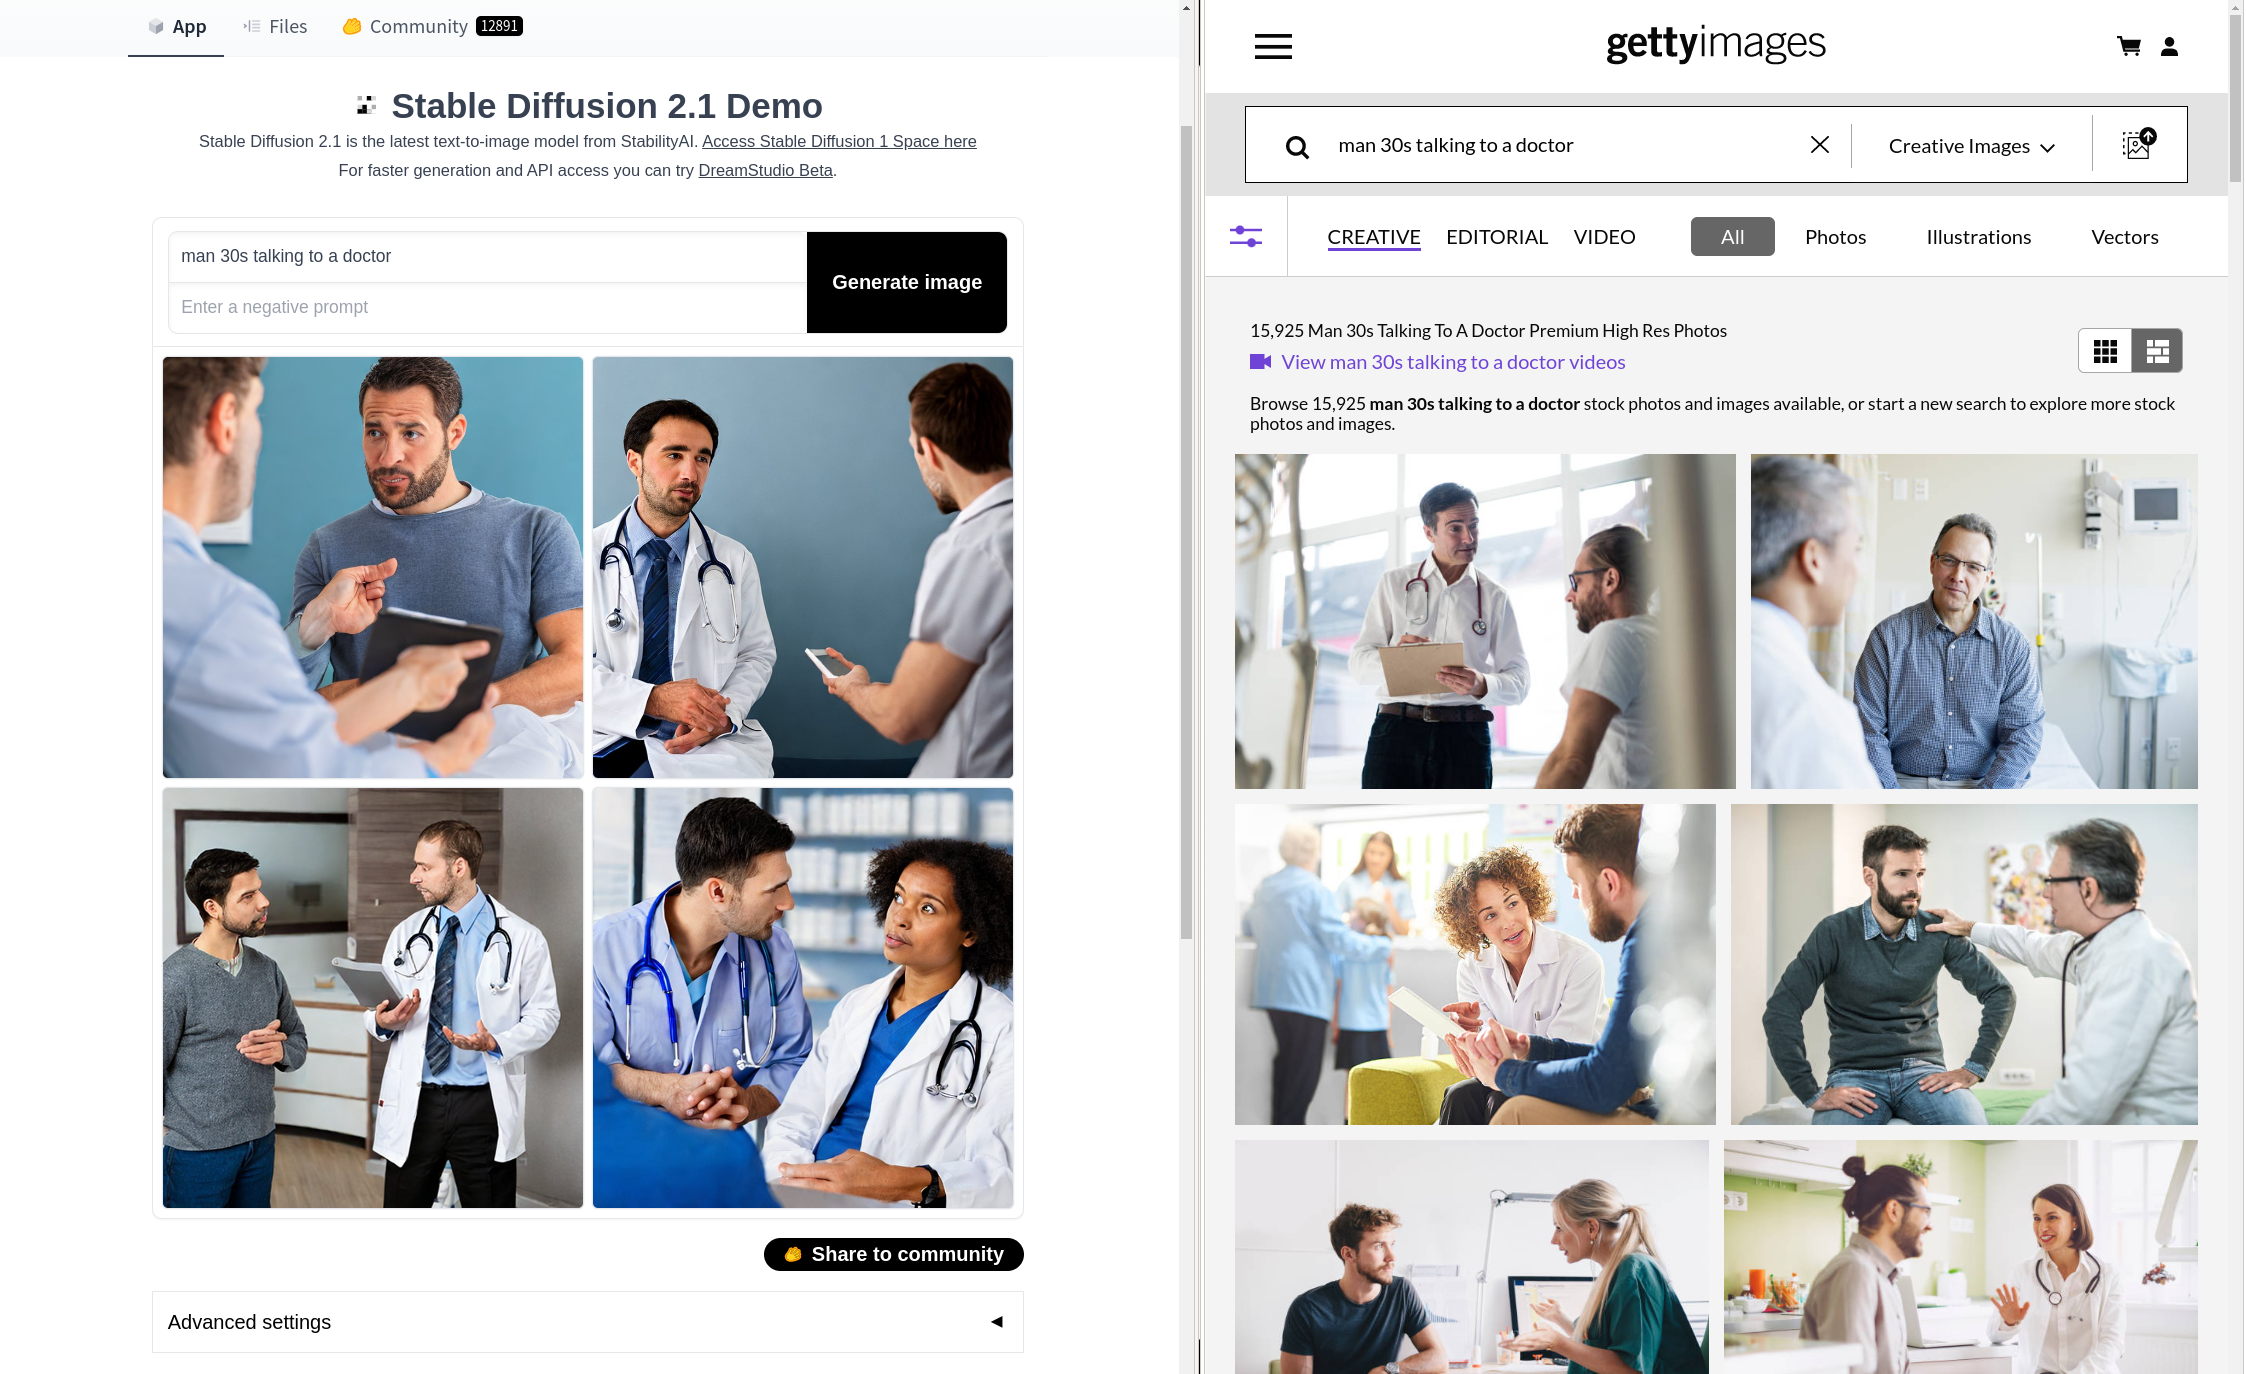
\includegraphics{getty}
        \caption{"man 30s talking to a doctor" Getty Images and Stable Diffusion comparison. Is Stable Diffusion creating something new here or spitting out it's training data? Is training a model like this fair use? I don't know, have fun lawyers! Note rights to each Getty photo runs around \$450, and Stable Diffusion is free to use, and they give users the rights to the model output. The Kraken has been released!}
        \labfig{getty}
\end{marginfigure}

These techniques can help to reduce the risk of having deep learning models reproduce the training data and cause intellectual property disputes, but there is no way to completely eliminate these risks, they are simply side-effects of the method of machine learning that we are doing nowadays. If you are an IP lawyer and need an expert witness, I'm your man \href{mailto:brad@bradflaugher.com}{brad@bradflaugher.com}.

\section{Working Together is Best}

It turns out sometimes the best combination is a reasonably smart (but not too cocky) human that gets to get recommendations from a few deep learning models. \sidenote{Funnily enough at Wharton I recently took \href{https://executiveeducation.wharton.upenn.edu/for-individuals/all-programs/effective-decision-making-thinking-critically-and-rationally/}{a class} where Dr. Cade Massey said basically "If you want to bring people along and get them to use your model, let them play with the output a bit, allowing for even the slightest bit (2\%) adjustment in the outputs will get users to adopt your model much faster." Thanks Cade!}

Garry Kasparov, the legendary chess player we heard about in chapter 1, witnessed a tournament where humans and AI could compete together. The tournament was designed to showcase the strengths of both humans and AI, and how they could work together to achieve incredible results here is what Garry says about the tournament:

\textit{"Once again, the chess world offers a useful test case for how this collaboration can play out. In 2005 the online chess playing site Playchess.com hosted what it called a "freestyle" chess tournament in which anyone could compete in teams with other players or computers. What made this competition interesting is that several groups of grandmasters working with computers also participated in this tournament. Predictably, most people expected that one of these grandmasters in combination with a supercomputer would dominate this competition ; but that's not what happened. The tournament was won by a pair of amateur American chess players using three computers. It was their ability to coordinate and coach effectively their computers that defeated the combination of a smart grandmaster and a PC with great computational power."}\sidecite{kasparov2005}

The tournament was a huge success, and showed that when humans and AI work together, they can achieve amazing things. The tournament participants learned that AI is not just a tool, but a valuable partner, and that by combining their strengths, they could achieve results that neither could have accomplished on their own. The tournament inspired many people to explore the potential of human-AI collaboration, and showed that by embracing technology, we can create a brighter future for all.

AI is an amazing partner, but we need to think for ourselves too. We can't blindly trust AI, but we can use it to inspire and challenge us.\sidecite{mansharamani2020}

\section{Key Takeaways}

\begin{itemize}
    \item \textbf{When you are using deep learning models, you are almost always engaging in some kind of transfer learning.} You are assuming the past will be like the future, or that training set reflects reality, which isn't always the case. \sidenote{It's as simple as the common financial disclaimer \textit{Past performance is no guarantee of future results.} Even though it is everywhere, the general public and even big swingers in finance don't seem to get this one. In AI there is an additional disclaimer, \textit{Training data may not reflect the the "real world".}}
    \item \textbf{Models can puke out seemingly creative things, but they are still a product of their training data.} deep learning models are deterministic systems, they slap together data based on rules they guessed from their training data. This process can still be very useful, but deep learning models are not sentient creative creatures from science fiction.
    \item \textbf{Even if you think you "own the rights" to the output of a model, models can sometimes puke out their training data} modelers try their best to prevent this but models can spit out their training data, which may cause headaches for everyone except the intellectual property lawyers. 
    \item \textbf{Users should consider the quality and appropriateness of the data the model they are using is trained on before deciding to use a model.} Remember, machine learning engineers spend most of their time cleaning up and gathering data, if you ask questions about how and when the data was collected and cleaned up you can get ahead of potential problems of concept drift and blind transfer learning (engaging in transfer learning without your consent).
    \item \textbf{Work with the technology} don't make your model do everything, sometimes it'll come up with stupid answers. Also don't assume you are always right, try and remember the story of the freestyle chess tournament and the grandmasters who got beat by the ameteurs getting reasonable advice from a few chess engines. Working with your model, as if it were a coworker that you don't fully trust, but still think is smart is probably the best way to use deep learning models.
\end{itemize}

